\documentclass[11pt]{article}

\usepackage[utf8]{inputenc}
\usepackage[english]{babel}
\usepackage[english]{isodate}
\usepackage[parfill]{parskip}

\usepackage{graphicx}
%%
% Just some sample text
\usepackage{lipsum}
\usepackage{tabularx}
\usepackage{xcolor} % for colour
\usepackage{colortbl}
%\usepackage{multirow}
\usepackage{lettrine}
\usepackage{csquotes}
\usepackage{placeins}

\usepackage{amsmath}
\usepackage{mathtools}
\usepackage{amssymb}
\usepackage{nccmath}
\usepackage{relsize}
\usepackage[sorting=none]{biblatex} %Imports biblatex package
\usepackage{tikz}
\usepackage{circuitikz}

\usepackage[colorlinks=true,allcolors=black]{hyperref}

\addbibresource{refs.bib} %Import the bibliography file

\usepackage{geometry}
 \geometry{
	a4paper,
	total={170mm,257mm},
	left=20mm,
	top=20mm,
}



\title{\textbf{Unbalanced power flow}}

\author{Josep Fanals i Batllori}



\begin{document}
	
	\maketitle

	The power flow problem is typically formulated under a set of hypothesis. Mainly, loads are balanced and lines are transposed. These assumptions are widely accepted for transmission systems. However, their validity starts suffering at the distribution level due to the presence of unbalances in the demand, the use of single-phase lines, non-transpositions, neutral conductors, etc. This document provides a modelling approach for distribution networks, and the subsequent power flow formulation required to handle such unbalanced systems. Initially, only the most common power system components are considered, such as loads, generators, transformers, and lines. 

	\section{Modelling}
	The main reference for modelling the main devices is the textbook "Distribution System Modeling and Analysis" by William H. Kersting~\cite{kersting2018distribution}.

	\subsection{Overhead lines}
	Overhead lines are those that are not buried underground. The general notation for an overhead line is shown in Figure~\ref{fig:ovline}, where it involves three phases, a neutral conductor, and ground.


	\begin{figure}[!htb]
		\centering
		\begin{circuitikz}[american]
			\draw[line width=0.7mm] (2,0) to [short] (2,-3);
			\draw[line width=0.7mm] (7,0) to [short] (7,-3);
			\draw (2,-0.5) to [short, i=$\underline{i}_a$] (7,-0.5);
			\draw (2,-1.5) to [short, i=$\underline{i}_b$] (7,-1.5);
			\draw (2,-2.5) to [short, i=$\underline{i}_c$] (7,-2.5);
			\draw (2.5,-3.5) to [short, i=$\underline{i}_n$] (6.5,-3.5);
			\draw (2.5,-3.5) to [short] (2.5,-4.5);
			\draw (6.5,-3.5) to [short] (6.5,-4.5);
			\node at (1.5,-0.5) {$\underline{v}_{fa}$};
			\node at (1.5,-1.5) {$\underline{v}_{fb}$};
			\node at (1.5,-2.5) {$\underline{v}_{fc}$};
			\node at (7.5,-0.5) {$\underline{v}_{ta}$};
			\node at (7.5,-1.5) {$\underline{v}_{tb}$};
			\node at (7.5,-2.5) {$\underline{v}_{tc}$};
			\draw (2.0,-4.5) to [short] (3.0,-4.5);
			\draw (6.0,-4.5) to [short] (7.0,-4.5);
			\draw (2.75,-4.5) to [short] (2.75,-5);
			\draw (6.25,-4.5) to [short] (6.25,-5);
			\draw (2.75,-5) to [short, i=$\underline{i}_g$] (6.25,-5);
			\node at (8.0,-4.2) {$\rho$};

			\draw[dashed] (0,-4) .. controls (2,-3.7) and (4,-3.9) .. (6,-3.8) 
								 .. controls (7,-3.7) .. (9,-4);
			\end{circuitikz}		
			\caption{Representation of an overhead line.}
			\label{fig:ovline}
	\end{figure}
	\FloatBarrier

	It is assumed that the neutral conductor is connected to ground on the two sides of the line. While this consideration may not always hold true, it is a common practice in conventional distribution systems (akin to the TT scheme in Spain). Also, the reference point for all voltage is the ground, with a resistivity denoted by $\rho$. The ground can be seen as a conductor as well. There is no conductor installed there per se, yet the ground has a finite electrical conductivity, 

	While transmission systems could be simplified to a single-phase model, distribution systems require a much more detailed model. In this sense, the voltage drop along a phase is caused by its current, but also by the rest of the currents. It is derived from Figure~\ref{fig:ovline} that a total of five currents has to be considered. The global relationship between currents and voltages can be established between impedances as:
	\begin{equation}
		\begin{pmatrix}
			\underline{v}_{fa} - \underline{v}_{ta} \\
			\underline{v}_{fb} - \underline{v}_{tb} \\
			\underline{v}_{fc} - \underline{v}_{tc} \\
			0 \\
			0 \\
		\end{pmatrix}
	= \begin{pmatrix}
		\underline{z}_{aa} & \underline{z}_{ab} & \underline{z}_{ac} & \underline{z}_{an} & \underline{z}_{ag} \\
		\underline{z}_{ba} & \underline{z}_{bb} & \underline{z}_{bc} & \underline{z}_{bn} & \underline{z}_{bg} \\
		\underline{z}_{ca} & \underline{z}_{cb} & \underline{z}_{cc} & \underline{z}_{cn} & \underline{z}_{cg} \\
		\underline{z}_{na} & \underline{z}_{nb} & \underline{z}_{nc} & \underline{z}_{nn} & \underline{z}_{ng} \\
		\underline{z}_{ga} & \underline{z}_{gb} & \underline{z}_{gc} & \underline{z}_{gn} & \underline{z}_{gg} \\
	\end{pmatrix}
	\begin{pmatrix}
		\underline{i}_{a} \\
		\underline{i}_{b} \\
		\underline{i}_{c} \\
		\underline{i}_{n} \\
		\underline{i}_{g} \\
	\end{pmatrix}.
	\label{eq:comp1}
	\end{equation}
	Diagonal impedance terms are caused by the self-impedance of the line (constituted by the resistance and the self-inductance of the line), whereas the off-diagonal terms are only due to the mutual impedance between phases. The diagonal term for the $m$ conductor, per unit length, is:
	\begin{equation}
			\underline{z}_{mm} = r_m + j 2\pi f 2\cdot 10^{-7} \ln \frac{1}{\text{GMR}_m}, 
	\end{equation}
	where $r_m$ is the resistance per unit length, $f$ is the frequency, and $\text{GMR}_m$ is the geometric mean radius of the conductor, roughly $r\cdot e^{-1/4}$, being $r$ the radius of such conductor. 
	
	The mutual impedance between two conductors $m$ and $k$ is given by:
	\begin{equation}
		\underline{z}_{mk} = j 2\pi f 2\cdot 10^{-7} \ln \frac{1}{D_{mk}},
	\end{equation}
	where $D_{mk}$ is the distance between conductors $m$ and $k$. 

	From the expressions above it can be inferred that computing the ground term is not straightforward, given its unknown radius and the undetermined distances between the active conductors and the core of the ground. Carson's equations were derived to circumvent such barriers and embed the ground in the model. Thus, the impedances are modified accounting for the effect of the ground. The equations that follow use the single-term approximation of Carson's original expressions~\cite{krolo2018computation}. These are found to be satisfactory to study low-frequency phenomena (such as the power flow being it a quasi-static problem). 
	
	Diagonal terms take the following form:
		\begin{equation}
			\underline{\hat{z}}_{mm} = r_m + j 2\pi f 2\cdot 10^{-7} \ln \frac{1}{\text{GMR}_m} + j\frac{\omega \mu_0}{2\pi}\ln \frac{D_e}{r} + \frac{\omega \mu_0}{8}, 
	\end{equation}
	where $\mu_0$ is the magnetic permeability of the vacuum, equal to $4\pi \cdot 10^{-7}$~H/m, and $D_e$ is given by:
	\begin{equation}
		D_e \approx 659 \sqrt{\frac{\rho}{f}}.
	\end{equation}

	Off-diagonal components are given by:	
	\begin{equation}
		\underline{\hat{z}}_{mk} = j 2\pi f 2\cdot 10^{-7} \ln \frac{1}{D_{mk}} + \frac{\omega \mu_0}{8} + j \frac{\omega \mu_0}{2\pi} \ln \frac{D_e}{D_{mk}}.
	\end{equation}
	The hat symbol is used to denote the modified impedance terms (also called primitive terms).

	More accurate expressions were proposed by Dubanton~\cite{dubanton1969calcul}, taking into account the distance between the conductors and ground, but at this stage the single-term approximation is deemed sufficient for the power flow problem.	

	With these transformations, the complete expression in~\eqref{eq:comp1} becomes:
	\begin{equation}
		\begin{pmatrix}
			\underline{v}_{fa} - \underline{v}_{ta} \\
			\underline{v}_{fb} - \underline{v}_{tb} \\
			\underline{v}_{fc} - \underline{v}_{tc} \\
			0 \\
		\end{pmatrix}
	= \begin{pmatrix}
		\underline{\hat{z}}_{aa} & \underline{\hat{z}}_{ab} & \underline{\hat{z}}_{ac} & \underline{\hat{z}}_{an} \\ 
		\underline{\hat{z}}_{ba} & \underline{\hat{z}}_{bb} & \underline{\hat{z}}_{bc} & \underline{\hat{z}}_{bn} \\
		\underline{\hat{z}}_{ca} & \underline{\hat{z}}_{cb} & \underline{\hat{z}}_{cc} & \underline{\hat{z}}_{cn} \\
		\underline{\hat{z}}_{na} & \underline{\hat{z}}_{nb} & \underline{\hat{z}}_{nc} & \underline{\hat{z}}_{nn} \\
	\end{pmatrix}
	\begin{pmatrix}
		\underline{i}_{a} \\
		\underline{i}_{b} \\
		\underline{i}_{c} \\
		\underline{i}_{n} \\
	\end{pmatrix}.
	\end{equation}

	% explain Kron reduction and how we end up with the 3x3
	


	\subsection{Loads}
	\subsection{Generators}
	\subsection{Transformers}

	\section{Power flow formulation}

	
	\section{Devices controls}
	This section unveils the controls associated with the most common devices found in power systems.

	\subsection{Load}
	% ZIP
	Loads are best represented with their equivalent ZIP model as shown in Figure~\ref{fig:load}.

	\begin{figure}[!htb]
		\centering
		\begin{circuitikz}[american]
			\draw[line width=0.7mm] (0,0) to [short] (7,0);
			\draw (0.6,0) to[generic, l=$G_i+jB_i$] (0.6,-3);
			\draw (3.5,0) to [isource, l=$I^\text{re}_i + jI^\text{im}_i$] (3.5,-3);
			\draw (6.4,0) to [cute european voltage source, l=$P_i+jQ_i$] (6.4,-3);
			\draw (0,-3) to [short] (7,-3);
			\end{circuitikz}		
			\caption{Representation of a load with its ZIP model.}
			\label{fig:load}
	\end{figure}
	\FloatBarrier


	\subsection{Generator}
	% include static gen. as PQ
	Under GridCal, generators are classified into two categories: controlled generators and static generators. The first category corresponds to the ones that regulate the voltage and the active power, whereas the second class contains generators setting a given active and reactive power.

	Figure~\ref{fig:gen_contr} shows the scheme for a controlled generator.

	\begin{figure}[!htb]
		\centering
		\begin{circuitikz}[american]
			\draw[line width=0.7mm] (2,0) to [short] (5,0);
			\draw (3.5,0) to [sV, l=$P_i$] (3.5,-3);
			\draw (2,-3) to [short] (5,-3);
			\node at (3.5,0.35) {$V_i$};
			\end{circuitikz}		
			\caption{Representation of a controlled generator.}
			\label{fig:gen_contr}
	\end{figure}
	\FloatBarrier

	Figure~\ref{fig:gen_stat} shows the scheme for a static generator.

	\begin{figure}[!htb]
		\centering
		\begin{circuitikz}[american]
			\draw[line width=0.7mm] (2,0) to [short] (5,0);
			\draw (3.5,0) to [sV, l=$P_i+jQ_i$] (3.5,-3);
			\draw (2,-3) to [short] (5,-3);
			\end{circuitikz}		
			\caption{Representation of a static generator.}
			\label{fig:gen_stat}
	\end{figure}
	\FloatBarrier
	Note that generators have a capability curve that limits their range of operation. Hence, it is common practice to switch a controlled generator to a static one in case the reactive power limits are met.
	
	\subsection{Shunt converter}  % a battery can be connected to it
	A shunt converter is understood as a device that links a resource (renewables, batteries, etc.) into the AC grid. Its model is captured in Figure~\ref{fig:vsc_shunt}.

	\begin{figure}[!htb]
		\centering
		\begin{circuitikz}[american]
			\draw[line width=0.7mm] (2,0) to [short] (5,0);
			\draw (3.5,0) to [sacdc, l=$P_i+jQ_i$] (3.5,-3);
			\draw (2,-3) to [short] (5,-3);
			\node at (3.5,0.35) {$V_i \angle \delta_i$};
			\node at (2.7, -1.5) {$I_i$};
			\end{circuitikz}		
			\caption{Representation of a shunt converter.}
			\label{fig:vsc_shunt}
	\end{figure}
	\FloatBarrier
	Seen from the AC side, a converter can control two magnitudes at a time, including the active and reactive powers, the voltage in magnitude and angle, and also operate at a set current magnitude. The operating mode determines the controlled variables.

	\subsection{Series converter}
	We define a series converter as a device of branch type, that is, a link between two buses where none of them is the ground. This kind of converter is found in HVDC links, for example. Figure~\ref{fig:vsc_series} displays its model. 

	\begin{figure}[!htb]
		\centering
		\begin{circuitikz}[american]
			\draw[line width=0.7mm] (2,0) to [short] (2,-3);
			\draw[line width=0.7mm] (7,0) to [short] (7,-3);
			\draw (2,-1.5) to [sacdc] (7,-1.5);
			\draw (4,-1.5) to [short, i_=$P_f+jQ_f$] (2,-1.5);
			\draw (5,-1.5) to [short, i=$P_t$] (7,-1.5);
			\node at (2,0.35) {$V_f \angle \delta_f$};
			\node at (7,0.35) {$V_t$};
			\node at (3,-2.0) {$I_f$};
			\end{circuitikz}		
			\caption{Representation of a series converter.}
			\label{fig:vsc_series}
	\end{figure}
	\FloatBarrier

	\subsection{Transformer}
	A transformer is seen as a device where its tap is adjustable, both in terms of magnitude and phase. In a simplified way its model is shown in Figure~\ref{fig:trafo}.

	\begin{figure}[!htb]
		\centering
		\begin{circuitikz}[american]
			\draw[line width=0.7mm] (2,0) to [short] (2,-3);
			\draw[line width=0.7mm] (7,0) to [short] (7,-3);
			\draw (2,-1.5) to [cute inductor, l=$m\angle \tau$] (7,-1.5);
			\draw (4,-1.5) to [short, i_=$P_f+jQ_f$] (2,-1.5);
			\draw (5,-1.5) to [short, i=$P_t+jQ_t$] (7,-1.5);
			\node at (2,0.35) {$V_f \angle \delta_f$};
			\node at (7,0.35) {$V_t \angle \delta_t$};
			\end{circuitikz}		
			\caption{Representation of a transformer.}
			\label{fig:trafo}
	\end{figure}
	\FloatBarrier


	\section{Fundamental rules}	
	There are some basic rules to ensure controls are coherent:

	\begin{itemize}
		\item Each grid has to have only 1 slack bus~\footnote{The only exception being distributed slacks, which are simply slack buses with coordination rules.}. This applies to both AC and DC grids. In AC grids the magnitude $V$ and angle $\delta$ have to be specified, whereas in DC grids only the magnitude $V$.
		\item It is not possible to have two devices controlling the same nodal voltage. In case it happens, there has to be a dominant device that governs it and the non-dominant device must switch its state.
		\item Buses can have from 0 to 4 controlled magnitudes. In the most extreme case, a device connected to a given bus may be controlling two magnitudes of a nearby bus (hence one bus has zero controlled magnitudes and the other four). Controlling 5 magnitudes is deemed impossible.
	\end{itemize}


\newpage
\section{Revisited power flow}
% P and Q eq.
% Pf and Pt eq. trafos and acdc
The traditional power flow problem considers three types of buses: slack, PQ and PV. The set of non-linear equations is solved for the voltage magnitudes and angles of the PQ and PV buses (as the slack is already set). However, this conventional formulation poses some challenges, such as:
\begin{itemize}
	\item Remote controls are not taken into account.
	\item No more than two magnitudes can be controlled in a given bus.
	\item Lack of consideration when it comes to controlled branch magnitudes.
	\item The bus type is predefined, which is not the case in the generalized power flow as there can be control switching.
	\item DC grids are not considered.
\end{itemize}
All these limitations are hindering the capability to model and solve modern grids. The generalized power flow is a step forward in this direction, as it allows for a more flexible and comprehensive approach to the power flow problem.

The adopted methodology has to be able to handle:
\begin{itemize}
	\item Remote controls and the possibility to control more than two magnitudes in a bus.
	\item Controlled branch magnitudes.
	\item Interconnected AC/DC grids to be solved in a unified manner.
	\item All potential bus types without explicitly defining them.
\end{itemize}
For this, we start by defining a general bus object with index $r$, such as indicated in Fig.~\ref{fig:busgen}.

\begin{figure}[!htb]
	\centering
	\begin{circuitikz}[american]
		\draw[line width=0.7mm] (0,0) to [short] (7,0);
		\draw (0.6,0) to[generic, l=$G_r+jB_r$] (0.6,-3);
		\draw (3.5,-3) to [isource, l_=$I^\text{re}_r + jI^\text{im}_r$] (3.5,-0);
		\draw (6.4,0) to [cute european voltage source, l=$P_r+jQ_r$] (6.4,-3);
		\draw (0,-3) to [short] (7,-3);
		\draw (2,0) to [short] (1,2);
		\draw (2.5,0) to [short] (1.75,2);
		\draw (3.0,0) to [short] (2.5,2);
		\draw (5,0) to [short] (6,2);
		\draw (4.5,0) to [short] (5.25,2);
		\draw (4.0,0) to [short] (4.5,2);
		\draw[dashed] (2,1) ellipse (1.2cm and 0.55cm);
		\draw[dashed] (5.0,1) ellipse (1.2cm and 0.55cm);

		\node at (6.6,1.0) {$\Gamma$};
		\node at (0.4,1.0) {$\kappa$};
		\node at (7.6, 0.0) {$V_r\angle \delta_r$};
		
		\end{circuitikz}		
		\caption{Representation of a generic bus with a ZIP shunt model, passive branch connections, and active branch connections.}
		\label{fig:busgen}
\end{figure}
\FloatBarrier
Branches belong to two sets:
\begin{itemize}
	\item $\kappa$: set of passive branches that can be represented through admittances. For example, power lines and non-controllable transformers are part of this set.
	\item $\Gamma$: set of branches interfaced to elements that cannot be inherently modelled through admittances, mainly AC/DC converters and controllable taps.
\end{itemize}
It is observed in Fig.~\ref{fig:busgen} that the ZIP model is employed to represent the shunt elements. This is a common practice in power systems, as it allows for a more accurate representation of the load. The ZIP model is given by three components: a constant admittance, a constant current source, and a constant power injection. The three components can be grouped under a ZIP power that takes the form:
\begin{equation}
	P_r^\text{zip} + jQ_r^\text{zip} = V_r^2(G_r-jB_r) + V_r\angle\delta_r(I_r^\text{re} - jI_r^\text{im}) + P_r + jQ_r.
\end{equation}
With this, by applying Kirchhoff laws, the nodal balance equation can be written as:
\begin{equation}
	0 = {V}Y^*_\text{bus}{V}^* + {C}_f^\Gamma({P}^\Gamma_f + j{Q}^\Gamma_f) + {C}_t^\Gamma({P}^\Gamma_t + j{Q}^\Gamma_t) - {P}^\text{zip} - j{Q}^\text{zip},
\end{equation}
where $Y_\text{bus}$ is the passive bus admittance matrix, and $C_f^\Gamma$ and $C_t^\Gamma$ are the from and to connectivity matrices of the set $\Gamma$. The set $\Gamma$ is the set of branches interfaced to elements that cannot be purely modelled with admittances, mainly AC/DC converters and controllable transformers. Hence, the powers $P^\Gamma_f$, $Q^\Gamma_f$, $P^\Gamma_t$, and $Q^\Gamma_t$ are the active and reactive powers of the branches belonging to this set. Notice that up to this point the only addition with respect to the conventional power flow is the presence of the set $\Gamma$ and the related objects.

Then, it is worth mentioning the employed models for all branches. A branch $b$ that belongs to the set $\kappa$ is modelled through the two by two admittance matrix of the form:
\begin{equation}
	Y_{b\in\kappa} = 
	\begin{bmatrix}
		Y_{ff} & Y_{ft} \\
		Y_{tf} & Y_{tt}
	\end{bmatrix},
\end{equation}
where $Y_{ff}$, $Y_{ft}$, $Y_{tf}$, and $Y_{tt}$ are the admittances of the branches seen from the combination of bused from $f$ and to $t$. The selection of what bus belongs to $f$ and what bus to $t$ is arbitrary and to be fully decided by the user. 

For example, in the case of a transformer, the admittance matrix is given by:
\begin{equation}
	Y_{b\in \kappa} = 
	\begin{bmatrix}
		\dfrac{Y_s + Y_{sh}}{m^2} & -\dfrac{Y_s}{me^{-j\tau}} \vspace{0.2cm} \\
		-\dfrac{Y_s}{me^{j\tau}} & Y_s + Y_{sh} \\
	\end{bmatrix},
\end{equation}
where $Y_s$ stands for the series admittance component, $Y_{sh}$ for the shunt admittance term, $m$ for the tap ratio, and $\tau$ for the phase shift angle. A similar expression is obtained for a regular power line. Note that modelling a transformer where the tap is controllable is part of the $\Gamma$ set.

Branches linking the bus to an active element that cannot be modelled through a combination of passive admittances are part of the $\Gamma$ set. The way to interface the bus with these active devices is through the branch power injections $P_f^\Gamma$, $Q_f^\Gamma$, $P_t^\Gamma$, and $Q_t^\Gamma$ and the connectivity matrices $C_f^\Gamma$ and $C_t^\Gamma$. Such an active device can have some interior equation defining its behavior. For instance, in an AC/DC converter, the active powers on the $f$ and $t$ sides are related through the power loss equation:
\begin{equation}
	P_f^\text{acdc} + P_t^\text{acdc} = a + b\frac{\sqrt{P_f^{2,\text{acdc}} + Q_f^{2,\text{acdc}}}}{V_f} + c\frac{P_f^{2,\text{acdc}} + Q_f^{2,\text{acdc}}}{V_f^2}.	
\end{equation}
where the convention is to use $f$ for the AC side and $t$ for the DC side. The parameters $a$, $b$, and $c$ are the coefficients of the power loss equation, and $P_f$ and $Q_f$ are the active and reactive powers on the AC side. 
 
For controllable transformers, it can be discussed if part of their model could be moved to the $\kappa$ set. This is because the transformer can be modelled through a combination of passive admittances and also controllable power injections. However, the tap ratio and the phase shift angle are not directly related to the admittances, and hence, for now, they are part of the $\Gamma$ set. The corresponding equations for a controllable transformer are:
\begin{equation}
	\begin{aligned}
		P_f^\text{tr} + jQ_f^\text{tr} = V_f^2 \frac{Y_s^* + Y_{sh}^*}{m^2} - V_fV_t^*\frac{Y_s^*}{me^{j\tau}}, \\
		P_t^\text{tr} + jQ_t^\text{tr} = V_t^2 (Y_s^* + Y_{sh}^*) - V_tV_f^*\frac{Y_s^*}{me^{-j\tau}}.
	\end{aligned}
\end{equation}
Fig.~\ref{fig:14bus} illustrates the concept of remote controls. In this case, the generator located in bus 6 controls the voltage magnitude at bus 13 $V_{13}$ through its injected power $P_6$, whereas the transformer between buses 4 and 9 adjusts its tap module $m_{49}$ to regulate the to power $P_{t,52}$ of the line located between buses 2 and 5. Although these associations between the controlled magnitudes and the related unknowns may not make the most sense in a real-world scenario, they have to be allowed in the generalized power flow.

\begin{figure}[!htb]\centering
   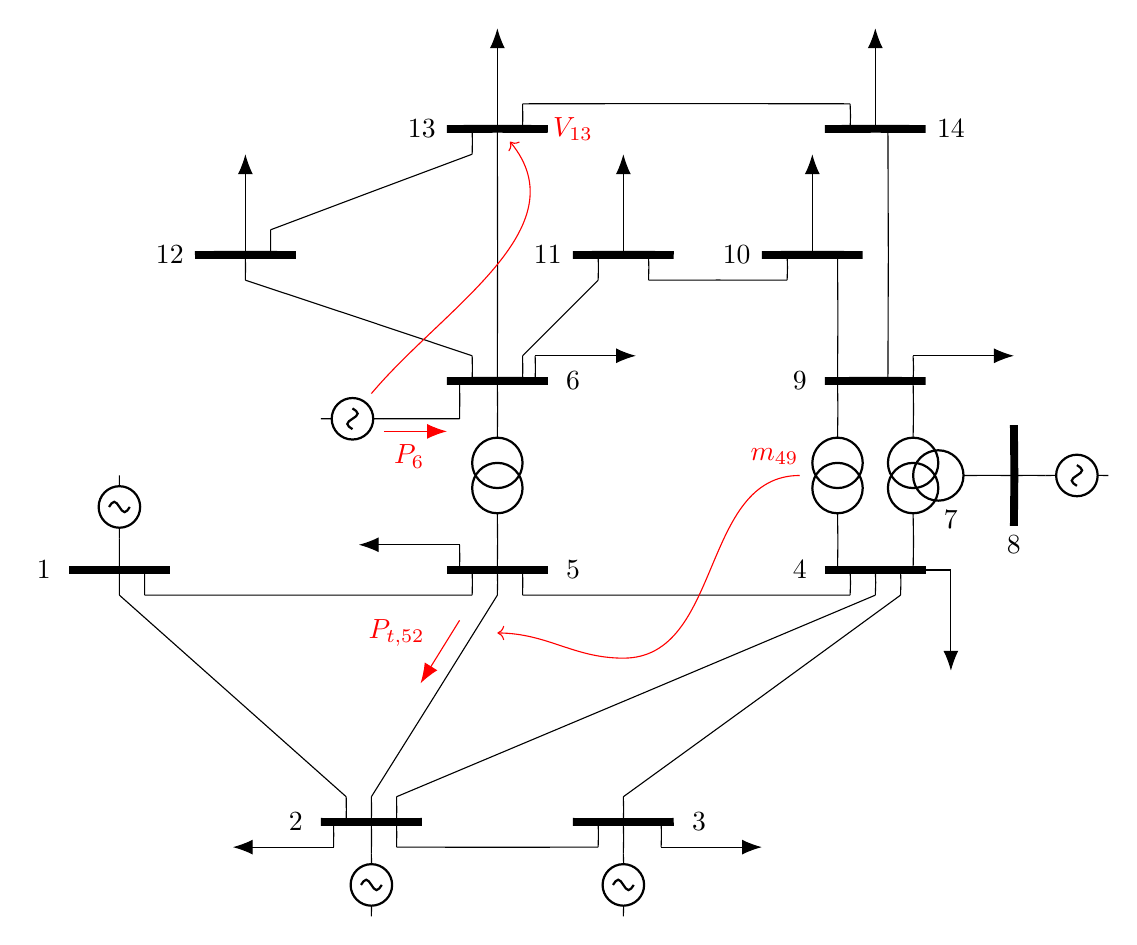
\begin{tikzpicture}[european, scale=1.6]

      % 0. Draw nodes
    \node(1) at (-0.2, 0) {1};
    \node(2) at (1.8, -2) {2};
    \node(3) at (5.0, -2) {3};
    \node(4) at (5.8, 0) {4};
    \node(5) at (4.0, 0) {5};
    \node(6) at (4.0, 1.5) {6};
    \node(7) at (7.0, 0.4) {7};
    \node(8) at (7.5, 0.2) {8};
    \node(9) at (5.8, 1.5) {9};
    \node(10) at (5.3, 2.5) {10};
    \node(11) at (3.8, 2.5) {11};
    \node(12) at (0.8, 2.5) {12};
    \node(13) at (2.8, 3.5) {13};
    \node(14) at (7.0, 3.5) {14};

    \node(p4) at (7.0, -1) {};
    \node(p5) at (2.1, 0.2) {};

      % 1. Draw buses
    \draw[line width=0.1cm] (0, 0) to [short] (0.8, 0);
    \draw[line width=0.1cm] (2, -2) to [short] (2.8, -2);
    \draw[line width=0.1cm] (6, 0) to [short] (6.8, 0);
    \draw[line width=0.1cm] (3, 0) to [short] (3.8, 0);
    \draw[line width=0.1cm] (4, -2) to [short] (4.8, -2);

    \draw[line width=0.1cm] (3, 1.5) to [short] (3.8, 1.5);
    \draw[line width=0.1cm] (6, 1.5) to [short] (6.8, 1.5);

    \draw[line width=0.1cm] (4.0, 2.5) to [short] (4.8, 2.5);
    \draw[line width=0.1cm] (5.5, 2.5) to [short] (6.3, 2.5);

    \draw[line width=0.1cm] (3, 3.5) to [short] (3.8, 3.5);
    \draw[line width=0.1cm] (6.0, 3.5) to [short] (6.8, 3.5);

    \draw[line width=0.1cm] (1.0, 2.5) to [short] (1.8, 2.5);
    \draw[line width=0.1cm] (7.5, 0.35) to [short] (7.5, 1.15);

    % 2. Draw trafos
    \draw[thick] (6.7, 0.65) circle (0.2cm);
    \draw[thick] (6.7, 0.85) circle (0.2cm);
    \draw[thick] (6.9, 0.75) circle (0.2cm);

    \draw[thick] (6.1, 0.65) circle (0.2cm);
    \draw[thick] (6.1, 0.85) circle (0.2cm);

    \draw[thick] (3.4, 0.65) circle (0.2cm);
    \draw[thick] (3.4, 0.85) circle (0.2cm);

    % 3. Draw generators
    \draw (0.4, 0.75) to [/tikz/circuitikz/bipoles/length=25pt, sinusoidal voltage source] (0.4,0.25);
    \draw (0.4, 0.25) to [short] (0.4,0); 

    \draw (2.4, -2.25) to [/tikz/circuitikz/bipoles/length=25pt, sinusoidal voltage source] (2.4, -2.75);
    \draw (2.4, -2.25) to [short] (2.4, -2.0); 

    \draw (4.4, -2.25) to [/tikz/circuitikz/bipoles/length=25pt, sinusoidal voltage source] (4.4, -2.75);
    \draw (4.4, -2.25) to [short] (4.4, -2.0); 

    \draw (7.75, 0.75) to [/tikz/circuitikz/bipoles/length=25pt, sinusoidal voltage source] (8.25, 0.75);
    \draw (7.75, 0.75) to [short] (7.5, 0.75); 

    \draw (2.0, 1.2) to [/tikz/circuitikz/bipoles/length=25pt, sinusoidal voltage source] (2.5, 1.2);
    \draw (2.5, 1.2) to [short] (3.1, 1.2); 
    \draw (3.1, 1.2) to [short] (3.1, 1.5); 

    % 4. Draw loads
    \draw (2.1, -2) to [short] (2.1, -2.2);
    \draw[-{Latex[scale=1.5]}] (2.1,-2.2) -- (1.3,-2.2);

    \draw (4.7, -2) to [short] (4.7, -2.2);
    \draw[-{Latex[scale=1.5]}] (4.7,-2.2) -- (5.5,-2.2);

    \draw (6.8, 0) to [short] (7.0, 0);
    \draw[-{Latex[scale=1.5]}] (7.0, 0) -- (7.0, -0.8);

    \draw (3.1, 0) to [short] (3.1, 0.2);
    \draw[-{Latex[scale=1.5]}] (3.1, 0.2) -- (2.3, 0.2);

    \draw (3.7, 1.5) to [short] (3.7, 1.7);
    \draw[-{Latex[scale=1.5]}] (3.7, 1.7) -- (4.5, 1.7);

    \draw (6.7, 1.5) to [short] (6.7, 1.7);
    \draw[-{Latex[scale=1.5]}] (6.7, 1.7) -- (7.5, 1.7);

    \draw[-{Latex[scale=1.5]}] (1.4, 2.5) -- (1.4, 3.3);
    \draw[-{Latex[scale=1.5]}] (3.4, 3.5) -- (3.4, 4.3);
    \draw[-{Latex[scale=1.5]}] (4.4, 2.5) -- (4.4, 3.3);
    \draw[-{Latex[scale=1.5]}] (5.9, 2.5) -- (5.9, 3.3);
    \draw[-{Latex[scale=1.5]}] (6.4, 3.5) -- (6.4, 4.3);

    % Draw lines
    \draw (0.4, 0) to [short] (0.4, -0.2);
    \draw (2.2, -2) to [short] (2.2, -1.8);
    \draw (0.4, -0.2) to [short] (2.2, -1.8);

    \draw (0.6, 0) to [short] (0.6, -0.2);
    \draw (3.2, 0) to [short] (3.2, -0.2);
    \draw (0.6, -0.2) to [short] (3.2, -0.2);
    
    \draw (3.4, 0) to [short] (3.4, -0.2);
    \draw (2.4, -2) to [short] (2.4, -1.8);
    \draw (3.4, -0.2) to [short] (2.4, -1.8);

    \draw (2.6, -2) to [short] (2.6, -2.2);
    \draw (4.2, -2) to [short] (4.2, -2.2);
    \draw (2.6, -2.2) to [short] (4.2, -2.2);

    \draw (2.6, -2) to [short] (2.6, -1.8);
    \draw (6.4, 0) to [short] (6.4, -0.2);
    \draw (2.6, -1.8) to [short] (6.4, -0.2);

    \draw (3.6, 0) to [short] (3.6, -0.2);
    \draw (6.2, 0) to [short] (6.2, -0.2);
    \draw (3.6, -0.2) to [short] (6.2, -0.2);

    \draw (4.4, -2) to [short] (4.4, -1.8);
    \draw (6.6, 0) to [short] (6.6, -0.2);
    \draw (4.4, -1.8) to [short] (6.6, -0.2);
    
    \draw (3.4, 0) to [short] (3.4, 0.45);
    \draw (3.4, 1.05) to [short] (3.4, 1.5);

    \draw (6.1, 0) to [short] (6.1, 0.45);
    \draw (6.1, 1.05) to [short] (6.1, 1.5);

    \draw (6.7, 0) to [short] (6.7, 0.45);
    \draw (6.7, 1.05) to [short] (6.7, 1.5);
    \draw (7.1, 0.75) to [short] (7.5, 0.75);
    
    \draw (1.4, 2.5) to [short] (1.4, 2.3);
    \draw (3.2, 1.5) to [short] (3.2, 1.7);
    \draw (1.4, 2.3) to [short] (3.2, 1.7);

    \draw (3.4, 1.5) to [short] (3.4, 3.5);

    \draw (3.6, 1.5) to [short] (3.6, 1.7);
    \draw (4.2, 2.5) to [short] (4.2, 2.3);
    \draw (3.6, 1.7) to [short] (4.2, 2.3);
    
    \draw (4.6, 2.5) to [short] (4.6, 2.3);
    \draw (5.7, 2.5) to [short] (5.7, 2.3);
    \draw (4.6, 2.3) to [short] (5.7, 2.3);
    
    \draw (6.1, 2.5) to [short] (6.1, 1.5);

    \draw (6.5, 1.5) to [short] (6.5, 3.5);
    
    \draw (6.2, 3.5) to [short] (6.2, 3.7);
    \draw (3.6, 3.5) to [short] (3.6, 3.7); 
    \draw (6.2, 3.7) to [short] (3.6, 3.7);
    
    \draw (1.6, 2.5) to [short] (1.6, 2.7);
    \draw (3.2, 3.5) to [short] (3.2, 3.3);
    \draw (1.6, 2.7) to [short] (3.2, 3.3);

	% Draw control arrows
	\draw[->, red] (5.8, 0.75) to [out=180, in=0] (4.4, -0.7) to [out=180, in=0] (3.4, -0.5);
	\draw[->, red] (2.4, 1.4) to [out=50, in=310] (3.5, 3.4); 

	\draw[-{Latex[scale=1.5]}, red] (2.5, 1.1) -- (3.0, 1.1);
	\draw[-{Latex[scale=1.5]}, red] (3.1, -0.4) -- (2.79, -0.9);
    \node[red](Pg6) at (2.7, 0.9) {$P_6$};
	\node[red](V13) at (4.0, 3.5) {$V_{13}$};
	\node[red](m49) at (5.6, 0.9) {$m_{49}$};
	\node[red](pt52) at (2.6, -0.5) {$P_{t,52}$};

  \end{tikzpicture}
  \caption{Scheme of the IEEE 14-bus system to illustrate the concept of remote controls.}
  \label{fig:14bus}
\end{figure}
From this, it follows that a set of known and unknown magnitudes has to be defined. The known magnitudes are the ones that are controlled, and the unknown magnitudes are the ones that are not controlled. The unknown set is composed of the following:
\begin{equation}
	x = [\delta, V, \tau, m, P^\text{zip}, Q^\text{zip}, P_f, P_t, Q_f, Q_t].
\end{equation}
Note that the conventional power flow formulation only contains the first two unknowns of the above defined $x$. This formulation includes many more unknowns, as it is designed to handle a broader range of cases, including regulated transformers, AC/DC links, among others.

The total number of equations to solve the system should be independent of the controls and resulting bus types. This is achieved by applying the nodal balance equations (both $P$ and $Q$) to the set of AC buses, the $P$ balance in all DC buses, the power loss equation for each AC/DC link, and the four power equations for each controlled transformer. Mathematically, in compact form:
\begin{equation}
	\begin{aligned}
		g_{p,ac} \coloneqq \sum P_i = 0 \quad \forall i \in AC, \\
		g_{q,ac} \coloneqq \sum Q_i = 0 \quad \forall i \in AC, \\
		g_{p,dc} \coloneqq \sum P_i = 0 \quad \forall i \in DC, \\
		g_{p,acdc} \coloneqq P_{fk}^\text{acdc} + P_{tk}^\text{acdc} - P_{\text{loss},k}^\text{acdc} = 0 \quad \forall k \in ACDC, \\
		g_{p_f,tr} \coloneqq P_{fk}^\text{tr} = f(\delta, V, \tau, m) \quad \forall k \in TR, \\
		g_{p_t,tr} \coloneqq P_{tk}^\text{tr} = f(\delta, V, \tau, m) \quad \forall k \in TR, \\
		g_{q_f,tr} \coloneqq Q_{fk}^\text{tr} = f(\delta, V, \tau, m) \quad \forall k \in TR, \\
		g_{q_t,tr} \coloneqq Q_{tk}^\text{tr} = f(\delta, V, \tau, m) \quad \forall k \in TR,
	\end{aligned}
\end{equation}
where $AC$ is the set of AC buses, $DC$ is the set of DC buses, $ACDC$ is the set of AC/DC links, and $TR$ is the set of controlled transformers. The index $i$ is employed to identify buses, while $k$ is employed to identify branches. 

Then, it is necessary to build arrays containing the indices where bus and branch magnitudes are either set of unknown. This is done through the sets $i$ to identify known bus magnitudes, $\overline{i}$ to identify unknown bus magnitudes, $k$ to identify known branch magnitudes, and $\overline{k}$ to identify unknown branch magnitudes. The sets are defined as shown in Table~\ref{tab:sets}. 

\begin{table}[!htb]
	\centering
	\caption{Sets to identify known and unknown magnitudes.}
	\begin{tabular}{cl}
		\hline
		\textbf{Set} & \textbf{Description} \\
		\hline
		$i_\delta$ & Known bus voltage phase \\
		$i_V$ & Known bus voltage magnitudes \\
		$i_p$ & Known bus ZIP active powers \\
		$i_q$ & Known bus ZIP reactive powers \\
		$k_\tau$ & Known branch tap phase shift angles \\
		$k_m$ & Known branch tap ratios \\
		$k_{p_f}$ & Known branch from active powers \\
		$k_{p_t}$ & Known branch to active powers \\
		$k_{q_f}$ & Known branch from reactive powers \\
		$k_{q_t}$ & Known branch to reactive powers \\
		$\overline{i}_\delta$ & Unknown bus voltage phase \\
		$\overline{i}_V$ & Unknown bus voltage magnitudes \\
		$\overline{i}_p$ & Unknown bus ZIP active powers \\
		$\overline{i}_q$ & Unknown bus ZIP reactive powers \\
		$\overline{k}_\tau$ & Unknown branch tap phase shift angles \\
		$\overline{k}_m$ & Unknown branch tap ratios \\
		$\overline{k}_{p_f}$ & Unknown branch from active powers \\
		$\overline{k}_{p_t}$ & Unknown branch to active powers \\
		$\overline{k}_{q_f}$ & Unknown branch from reactive powers \\
		$\overline{k}_{q_t}$ & Unknown branch to reactive powers \\
		\hline
	\end{tabular}
	\label{tab:sets}
\end{table}
The set of non-linear equations is meant to be solved with the Newton-Raphson method, where the Jacobian matrix is built from the partial derivatives of the equations with respect to the unknowns. In its general form, at each iteration the following linear system has to be solved:
\setlength{\arraycolsep}{1.5pt}
\begin{equation}
	-
	\begin{bmatrix}
		g_{p,ac} \\
		g_{q,ac} \\
		g_{p,dc} \\
		g_{p,acdc} \\
		g_{p_f,tr} \\
		g_{p_t,tr} \\
		g_{q_f,tr} \\
		g_{q_t,tr} \\
	\end{bmatrix} = 
	\begin{bmatrix}
		\frac{\partial g_{p,ac}}{\partial \delta} & \frac{\partial g_{p,ac}}{\partial V} & \frac{\partial g_{p,ac}}{\partial \tau} & \frac{\partial g_{p,ac}}{\partial m} & \frac{\partial g_{p,ac}}{\partial P^\text{zip}} & \frac{\partial g_{p,ac}}{\partial Q^\text{zip}} & \frac{\partial g_{p,ac}}{\partial P_f} & \frac{\partial g_{p,ac}}{\partial P_t} & \frac{\partial g_{p,ac}}{\partial Q_f} & \frac{\partial g_{p,ac}}{\partial Q_t} \\
		\frac{\partial g_{q,ac}}{\partial \delta} & \frac{\partial g_{q,ac}}{\partial V} & \frac{\partial g_{q,ac}}{\partial \tau} & \frac{\partial g_{q,ac}}{\partial m} & \frac{\partial g_{q,ac}}{\partial P^\text{zip}} & \frac{\partial g_{q,ac}}{\partial Q^\text{zip}} & \frac{\partial g_{q,ac}}{\partial P_f} & \frac{\partial g_{q,ac}}{\partial P_t} & \frac{\partial g_{q,ac}}{\partial Q_f} & \frac{\partial g_{q,ac}}{\partial Q_t} \\
		\frac{\partial g_{p,dc}}{\partial \delta} & \frac{\partial g_{p,dc}}{\partial V} & \frac{\partial g_{p,dc}}{\partial \tau} & \frac{\partial g_{p,dc}}{\partial m} & \frac{\partial g_{p,dc}}{\partial P^\text{zip}} & \frac{\partial g_{p,dc}}{\partial Q^\text{zip}} & \frac{\partial g_{p,dc}}{\partial P_f} & \frac{\partial g_{p,dc}}{\partial P_t} & \frac{\partial g_{p,dc}}{\partial Q_f} & \frac{\partial g_{p,dc}}{\partial Q_t} \\
		\frac{\partial g_{p,acdc}}{\partial \delta} & \frac{\partial g_{p,acdc}}{\partial V} & \frac{\partial g_{p,acdc}}{\partial \tau} & \frac{\partial g_{p,acdc}}{\partial m} & \frac{\partial g_{p,acdc}}{\partial P^\text{zip}} & \frac{\partial g_{p,acdc}}{\partial Q^\text{zip}} & \frac{\partial g_{p,acdc}}{\partial P_f} & \frac{\partial g_{p,acdc}}{\partial P_t} & \frac{\partial g_{p,acdc}}{\partial Q_f} & \frac{\partial g_{p,acdc}}{\partial Q_t} \\
		\frac{\partial g_{p_f,tr}}{\partial \delta} & \frac{\partial g_{p_f,tr}}{\partial V} & \frac{\partial g_{p_f,tr}}{\partial \tau} & \frac{\partial g_{p_f,tr}}{\partial m} & \frac{\partial g_{p_f,tr}}{\partial P^\text{zip}} & \frac{\partial g_{p_f,tr}}{\partial Q^\text{zip}} & \frac{\partial g_{p_f,tr}}{\partial P_f} & \frac{\partial g_{p_f,tr}}{\partial P_t} & \frac{\partial g_{p_f,tr}}{\partial Q_f} & \frac{\partial g_{p_f,tr}}{\partial Q_t} \\
		\frac{\partial g_{p_t,tr}}{\partial \delta} & \frac{\partial g_{p_t,tr}}{\partial V} & \frac{\partial g_{p_t,tr}}{\partial \tau} & \frac{\partial g_{p_t,tr}}{\partial m} & \frac{\partial g_{p_t,tr}}{\partial P^\text{zip}} & \frac{\partial g_{p_t,tr}}{\partial Q^\text{zip}} & \frac{\partial g_{p_t,tr}}{\partial P_f} & \frac{\partial g_{p_t,tr}}{\partial P_t} & \frac{\partial g_{p_t,tr}}{\partial Q_f} & \frac{\partial g_{p_t,tr}}{\partial Q_t} \\
		\frac{\partial g_{q_f,tr}}{\partial \delta} & \frac{\partial g_{q_f,tr}}{\partial V} & \frac{\partial g_{q_f,tr}}{\partial \tau} & \frac{\partial g_{q_f,tr}}{\partial m} & \frac{\partial g_{q_f,tr}}{\partial P^\text{zip}} & \frac{\partial g_{q_f,tr}}{\partial Q^\text{zip}} & \frac{\partial g_{q_f,tr}}{\partial P_f} & \frac{\partial g_{q_f,tr}}{\partial P_t} & \frac{\partial g_{q_f,tr}}{\partial Q_f} & \frac{\partial g_{q_f,tr}}{\partial Q_t} \\
		\frac{\partial g_{q_t,tr}}{\partial \delta} & \frac{\partial g_{q_t,tr}}{\partial V} & \frac{\partial g_{q_t,tr}}{\partial \tau} & \frac{\partial g_{q_t,tr}}{\partial m} & \frac{\partial g_{q_t,tr}}{\partial P^\text{zip}} & \frac{\partial g_{q_t,tr}}{\partial Q^\text{zip}} & \frac{\partial g_{q_t,tr}}{\partial P_f} & \frac{\partial g_{q_t,tr}}{\partial P_t} & \frac{\partial g_{q_t,tr}}{\partial Q_f} & \frac{\partial g_{q_t,tr}}{\partial Q_t} \\
	\end{bmatrix}
	\begin{bmatrix}
		\Delta \delta \\
		\Delta V \\
		\Delta \tau \\
		\Delta m \\
		\Delta P^\text{zip} \\
		\Delta Q^\text{zip} \\
		\Delta P_f \\
		\Delta P_t \\
		\Delta Q_f \\
		\Delta Q_t \\
	\end{bmatrix}
\end{equation}
	
	
\section{Bibliography}
	\printbibliography
	
\end{document}